% !TEX encoding = UTF-8 Unicode

\documentclass[a4paper]{article}

\usepackage{color}
\usepackage{url}
\usepackage[utf8]{inputenc}
\usepackage{graphicx}
\usepackage[english,serbian]{babel}
\usepackage[unicode]{hyperref}
\usepackage{amsmath}
\DeclareMathOperator{\arctantwo}{arctan2}
\usepackage{amsthm}
\usepackage{amssymb}
\hypersetup{colorlinks,citecolor=green,filecolor=green,linkcolor=blue,urlcolor=blue}
\usepackage[title]{appendix}
\usepackage{float}
\usepackage[graphicx]{realboxes}
\usepackage[font=small,labelfont=bf]{caption}
\usepackage{chngcntr}
\counterwithin{figure}{section}
\usepackage{listings}
\usepackage{textcomp}
\usepackage{xcolor}
\lstset {
    language=csh,
    frame=single,
    framesep=10pt,
    tabsize=4,
    xrightmargin=-25pt,
    showstringspaces=false,
    upquote=true,
    commentstyle=\color{commentgreen},
    keywordstyle=\color{blue},
    stringstyle=\color{red},
    basicstyle=\small\ttfamily,
    emphstyle={\color{blue}},
    escapechar=\&,
    % keyword highlighting
    classoffset=1, % starting new class
    morekeywords={ abstract, event, new, struct,
    as, explicit, null, switch,
    base, extern, object, this,
    bool, false, operator, throw,
    break, finally, out, true,
    byte, fixed, override, try,
    case, float, params, typeof,
    catch, for, private, uint,
    char, foreach, protected, ulong,
    checked, goto, public, unchecked,
    class, if, readonly, unsafe,
    const, implicit, ref, ushort,
    continue, in, return, using,
    decimal, int, sbyte, virtual,
    default, interface, sealed, volatile,
    delegate, internal, short, void,
    do, is, sizeof, while,
    double, lock, stackalloc,
    else, long, static,
    enum, namespace, string, 
    >,<,.,;,,,-,!,=,~},
    keywordstyle=\color{blue},
    classoffset=0,
}

\theoremstyle{plain}
\newtheorem{thm}{Teorema}[section]
\theoremstyle{definition}
\newtheorem{defn}[thm]{Definicija}
\newtheorem{exmp}[thm]{Primer}
\newtheorem{assn}[thm]{Pretpostavka}
\newtheorem{obsn}[thm]{Zapa\v{z}anje}
\newtheorem{prob}[thm]{Problem}


\begin{document}

\title{Korišćenje Furijeovih redova za crtanje pomoću epiciklusa\\ \small{Seminarski rad u okviru kursa\\Nau\v{c}no izra\v{c}unavanje\\ Matematički fakultet}}

\author{\href{mailto:ivan_ristovic@math.rs}{Ivan Ristovi\'c}}
\date{septembar 2019.}

\maketitle

\abstract{
    Najjednostavniji epiciklus predstavlja krug \v{c}iji se centar kre\'c{}e po kru\v{z}nici drugog kruga. Slo\v{z}eni epiciklusi nastaju rekurzivnim dodavanjem krugova u pomenuti sistem. Epiciklusi su poznati jo\v{s} od vremena starih Grka i kori\v{s}\'c{}eni su da opi\v{s}u slo\v{z}ena kretanja nebeskih tela. Pokazano je da se slaganjem dovoljnog broja epiciklusa odgovaraju\'c{}ih dimenzija i njihovim kretanjem odgovaraju\'c{}im brzinama mogu iscrtati najrazli\v{c}itije orbite bez obzira na njihovu slo\v{z}enost. U ovom radu se opisuje veza izmedju epiciklusa i diskretne Furijeove transformacije i ista se koristi za crtanje proizvoljnih neprekidnih linija daju\'c{}i fascinantno geometrijsko shvatanje Furijeove transformacije koje se krilo u epiciklusima poznatim od davnina.
}

\tableofcontents

\newpage

\section{Uvod}
\label{sec:Intro}

\subsection{Furijeova transformacija}
\label{sec:Fourier}

\emph{Furijeova transformacija} \cite{Fourier} razla\v{z}e funkciju u vremenskom domenu (tzv. \emph{signal}) u frekvencije od kojih je sa\v{c}injena. Tradicionalna oznaka za Furijeovu transformaciju funkcije $f$ je $\hat{f}$.

Neka je funkcija $f$ periodi\v{c}na na intervalu $[a,b]$ \footnote{U definiciji neprekidne Furijeove transformacije takodje pretpostavljamo da je $f$ integrabilna sa kvadratom na intervalu $[a,b]$}. Tada se $f$ mo\v{z}e razviti u \emph{Furijeov red} \cite{NI}:
$$f(t) = \frac{a_0}{2} \sum_{k=1}^{\infty}{a_k \cos{\frac{2\pi kt}{b-a}} + \sin{\frac{2\pi kt}{b-a}}}$$
gde va\v{z}i:
$$a_k = \frac{2}{b-a}\int_{a}^{b}{f(t)\cos{\frac{2\pi kt}{b-a}}dt}   , k = 0, 1, \dots$$
$$b_k = \frac{2}{b-a}\int_{a}^{b}{f(t)\sin{\frac{2\pi kt}{b-a}}dt}   , k = 1, 2, \dots$$

U praksi, signal je obi\v{c}no diskretan, pa se neprekidni Furijeov red zamenjuje diskretnom varijantom. Takodje, mogu\'c{}e je formirati kompleksnu reprezentaciju Furijeovog reda koriste\'c{}i jednakosti:
$$e^{i\theta} = \cos{\theta} + i\sin{\theta}$$
$$\cos{\theta} = \frac{e^{i\theta} + e^{-i\theta}}{2}$$
$$\sin{\theta} = i\frac{e^{-i\theta} - e^{i\theta}}{2}$$

Takva kompleksna reprezentacija Furijeovog reda \'c{}e biti kori\v{s}\'c{}ena kasnije u implementaciji, u narednoj formi:
$$\hat{f}_k = \frac{1}{n}\sum_{j=0}^{n}{c_je^{2\pi ikj/n}}, k = 0, 1, \dots, n-1$$
\subsection{Epiciklusi}
\label{sec:Epicycles}

Re\v{c} \emph{epiciklus}, u prevodu sa gr\v{c}kog, zna\v{c}i \emph{na krugu}, tj. \emph{krug na krugu}. Formalno, to je geometrijski model kori\v{s}\'c{}en da objasni varijacije u brzini i smeru kretanja Sunca, Meseca i ostalih planeta. Takav model je od gr\v{c}kih astronoma preuzeo i unapredio Ptolomej \footnote{Ptolomejev model je, kao i ostali modeli pre njega, pretpostavljao da je Zemlja u centru svemira. Medjutim, uprkos o\v{c}ito pogre\v{s}noj pretpostavci, njegov model je prvi precizno objasnio kretanje svemirskih tela}. Po Ptolomeju \cite{PtolemaicModel}, svaka planeta se kre\'c{}e po manjoj kru\v{z}noj putanji, zvanoj \emph{epiciklus}, dok se ta putanja kre\'c{}e po ve\'c{}oj kru\v{z}noj putanji, zvanoj \emph{deterent} (videti sliku \ref{img:PtolemaicModel}). 

\begin{figure}
    \centering
    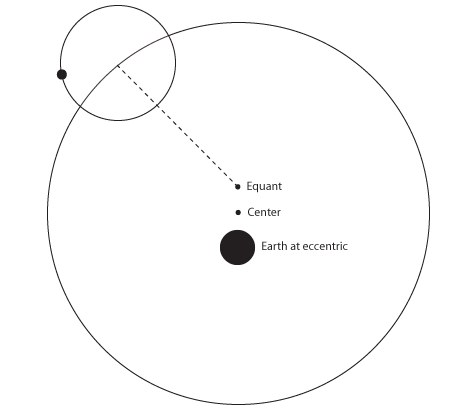
\includegraphics[scale=0.5]{images/ptolomaic_model.PNG}
    \caption{Ptolomejev model kretanja svemirskih tela.}
    \label{img:PtolemaicModel}
\end{figure}

Epicikluse mo\v{z}emo zakomplikovati rekurzivnim dodavanjem drugih epiciklusa. Dodati krugovi ne moraju (i \v{c}esto u primenama nisu) istih dimenzija. Postoje tvrdnje da je Ptolomejev model imao u opisima kretanja nekih planeta i do 80 epiciklusa, u poredjenju sa Kopernikovim sistemom, koji je imao do 34 epiciklusa \footnote{Nikola Kopernik je za cilj imao da smanji kompleksnost Ptolomejevog modela, \v{s}to je i uspeo u svom heliocentri\v{c}nom sistemu.}. Pokazano je da se bilo kakva putanja - bilo periodi\v{c}na ili ne, zatvorena ili otvorena - mo\v{z}e proizvoljno dobro aproksimirati \emph{slaganjem} dovoljnog mnogo epiciklusa odgovaraju\'c{}ih dimenzija (videti sliku \ref{img:pi}). U literaturi se takodje \v{c}esto za orbitu koju pravi poslednji krug koristi termin \emph{epiciklus}.

\begin{figure}
    \centering
    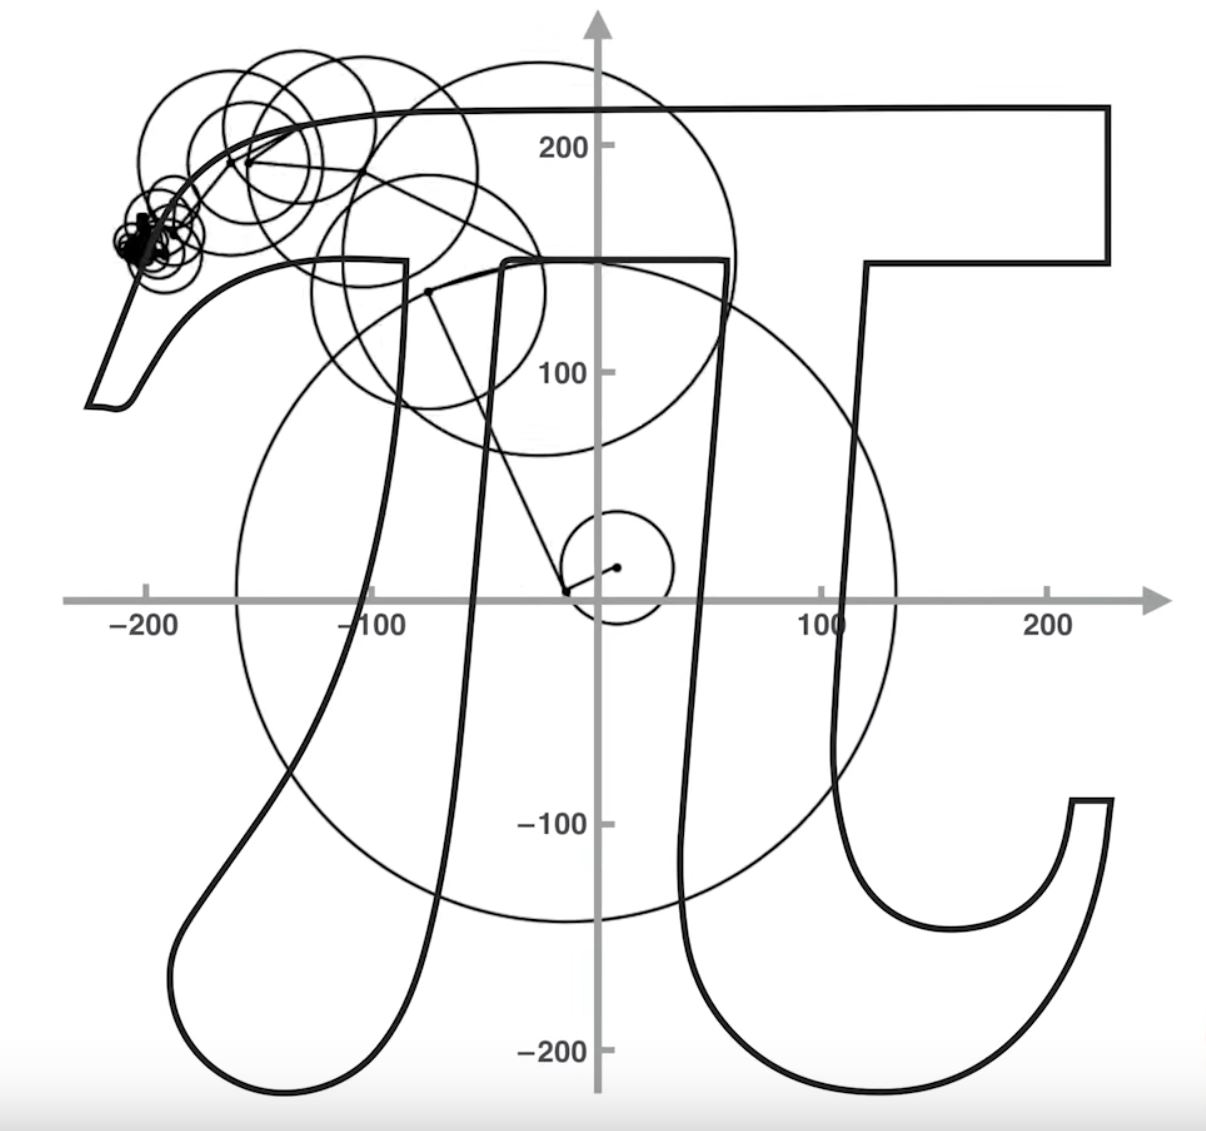
\includegraphics[scale=0.2]{images/pi.jpg}
    \caption{Demonstracija pra\'c{}enja orbite simbola $\pi$ pomo\'c{}u epiciklusa.}
    \label{img:pi}
\end{figure}

Epiciklusi se, naravno, mogu predstaviti potpuno formalno matemati\v{c}kim formulama. Deferent mo\v{z}emo predstaviti kao kompleksan broj
$$z_0 = a_0e^ik_0t,$$
gde su $a_0$ i $k_0$ konstante, $i$ imaginarna jedinica, a $t$ vreme. Deferent je stoga centriran u koordinatnom po\v{c}etku kompleksne ravni, sa polupre\v{c}nikom $a_0$ i ugaonom brzinom $k_0$ sa periodom $T$:
$$k_0 = \frac{2\pi}{T}.$$ 
Ukoliko je $z_1$ epiciklus, onda zbir deferenta i epiciklusa predstavlja periodi\v{c}nu funkciju \footnote{Zapravo, ovakve funkcije se nazivaju \emph{skoro periodi\v{c}ne funkcije} - zainteresovani \v{c}italac mo\v{z}e pro\v{c}itati vi\v{s}e u \cite{AlmostPeriodicFunctions}. Ova funkcija je periodi\v{c}na samo kada je udeo konstanti $k_j$ racionalan.}
$$z_2 = z_0 + z_1 = a_0e^ik_0t + a_1e^ik_1t.$$
Generalizovanjem dobijamo op\v{s}ti \v{c}lan:
$$z_n = \sum_{j=0}^{n}{a_je^ik_jt}$$

Postavlja se pitanje: \textit{\v{S}ta je zapravo putanja koju najmanji epiciklus pravi, i gde se ona krije u ovoj formuli}? Problem pronala\v{z}enja \emph{orbite} najmanjeg epiciklusa se sastoji u pronala\v{z}enju vrednosti koeficijenata $a_j$ kako bi se reprezentovao vremenski zavisan put u kompleksnoj ravni. Vi\v{s}e o tome u poglavljima koja slede.


\section{Crtanje proizvoljnih kontura}
\label{sec:Drawing}

Epiciklusi se mogu posmatrati kao krive definisane slede\'c{}im jedna\v{c}inama:
\begin{equation}
\begin{aligned} 
    x(t) & = \sum_i^N R_i\cos(\omega_i t + \phi_i)\\ 
    y(t) & = \sum_i^N R_i\sin(\omega_i t + \phi_i)\\ 
\end{aligned}
\label{eq:ep}
\end{equation}
gde $N$ predstavlja broj krugova u epiciklusu, $R_i$ predstavlja radijus kruga $i$, $\omega_i$ predstavlja ugaonu brzinu pridru\v{z}enu krugu $i$, a $\phi_i$ ozna\v{c}ava za koliki ugao je krug $i$ zarotiran u trenutku $t = 0$ (u daljem tekstu \emph{fazni pomeraj}).

Postavlja se pitanje: \emph{Kakve sve oblike, tj. orbite, mo\v{z}emo opisati epiciklusima}? Iz odeljka \ref{sec:Epicycles} znamo da se bilo kakva neprekidna linija mo\v{z}e opisati epiciklusom, pa \v{c}ak i prave linije ukoliko su krugovi istih dimenzija i rotiraju se u suprotnim smerovima tako da se $y$ komponente poni\v{s}tavaju (videti sliku \ref{img:line}). Jedini problem je zapravo odrediti vrednosti za $R$, $\omega$ i $\phi$ tako da prate proizvoljnu orbitu.

\begin{figure}
    \centering
    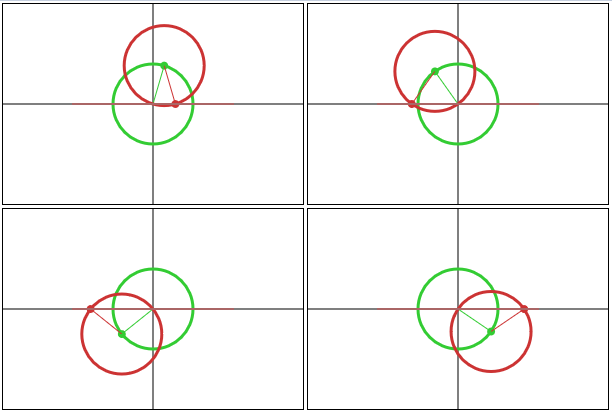
\includegraphics[scale=0.7]{images/line.PNG}
    \caption{Iscrtavanje prave linije zahteva samo dva kruga.}
    \label{img:line}
\end{figure}


\subsection{Ra\v{c}unanje epiciklusa za datu orbitu}

Najpre formalizujmo problem. Signal je dostupan u diskretnom obliku, kao skup ta\v{c}aka $(x_j,y_j)$. Zadatak je prona\'c{}i epicikluse tako da se date ta\v{c}ke najbolje spoje. Ta\v{c}nije, tra\v{z}imo $R_i$, $\omega_i$ i $\phi_i$ tako da $x(t)$ i $y(t)$ iz jednakosti \ref{eq:ep} \v{s}to bli\v{z}e odgovaraju signalu. $R_i$, $\omega_i$ i $\phi_i$ se onda mogu dobiti re\v{s}avanjem odgovaraju\'c{}eg sistema jedna\v{c}ina.

Prime\'c{}ujemo da u formalizaciji problema moramo \emph{pribli\v{z}iti} aproksimaciju signalu. To se mo\v{z}e formalizovati na razne na\v{c}ine, naj\v{c}e\v{s}\'c{}e pojmom \emph{srednjekvadratne gre\v{s}ke} \cite{NI}.

Ukoliko posmatramo ta\v{c}ke kao kompleksne brojeve, mogu\'c{}e je iskoristiti Ojlerovu formulu,
$$e^ix = \cos x + i\sin x,$$
i DFT proceduru opisanu u \ref{sec:Fourier} kako bismo kreirali algoritam koji je veoma jednostavan za ra\v{c}unar. Najpre formirajmo kompleksni broj koriste\'c{}i jedna\v{c}ine \ref{eq:ep}:
$$p_j = x_j + iy_j \\ x(t) + iy(t) = \sum_i^N R_i(\cos(\omega_i t + \phi_i) + i\sin(\omega_i t + \phi_i)).$$

Prime\'c{}ujemo da nismo ni\v{s}ta izgubili prelaskom na kompleksnu reprezentaciju, naime $x$ i $y$ su zapravo realni i imaginarni deo komplesnog re\v{s}enja. Sada, uz pomo\'c{} Ojlerove formule, shvatamo da tra\v{z}imo promenljive takve da izraz
$$\sum_j^N R_je^{i\omega_j t+ \phi_j}$$
\v{s}to bli\v{z}e odgovara kompleksnim brojevima $p_j$. \v{S}tavi\v{s}e, ukoliko dozvolimo da $X_j$ bude kompleksan broj, izraz postaje:
$$\sum_j^N X_je^{i\omega_j t}$$

Radi simplifikacije, umesto biranja $N$ ugaonih brzina $\omega$, postavi\'c{}emo fiksne brzine: $0, 1x, -1x, 2x, -2x, \dots , N/2x, -N/2x$. Sa ovom pretpostavkom, problem poprima finalni oblik:

\begin{prob}
    Prona\'c{}i kompleksne brojeve $X_j$ (krugove epiciklusa) minimizuju\'c{}i srednjekvadratnu gre\v{s}ku izmedju kompleksnih ta\v{c}aka $p_j$ i krive
    $$p(t) = \sum_{j=0}^N X_je^{\frac{2\pi i j}{N}t}.$$
\end{prob}

Problem opisan iznad skoro u potpunosti odgovara DFT formi. Stoga, dovoljno je iskoristiti DFT algoritam (videti \ref{sec:appendix:dft}), dobiti kompleksne brojeve $X_j$ i zatim izra\v{c}unati nepoznate parametre:
$$R_j = |X_j|,$$
$$\omega_j = \frac{2 \pi i j}{N},$$
$$\phi_j = \arctantwo(\Im{X_j}, \Re{X_j}).$$

\section{Implementacija}
\label{sec:impl}

Program koji automatizuje proces opisan u poglavlju \ref{sec:Drawing} je dostupan na GitHub-u: \url{https://github.com/ivan-ristovic/epicyclez}. Implementiran u \texttt{C\#}-u 7.3, trenutno dostupan samo za \texttt{Windows} operativni sistem \footnote{Sa izdanjem 3.0 .NET Core radnog okvira, program \'c{}e biti mogu\'c{}e pokrenuti na svim operativnim sistemima koji imaju instaliran .NET Core Runtime.}. Prikaz rada programa se mo\v{z}e videti na slici \ref{fig:impl}.

\begin{figure}
    \centering
    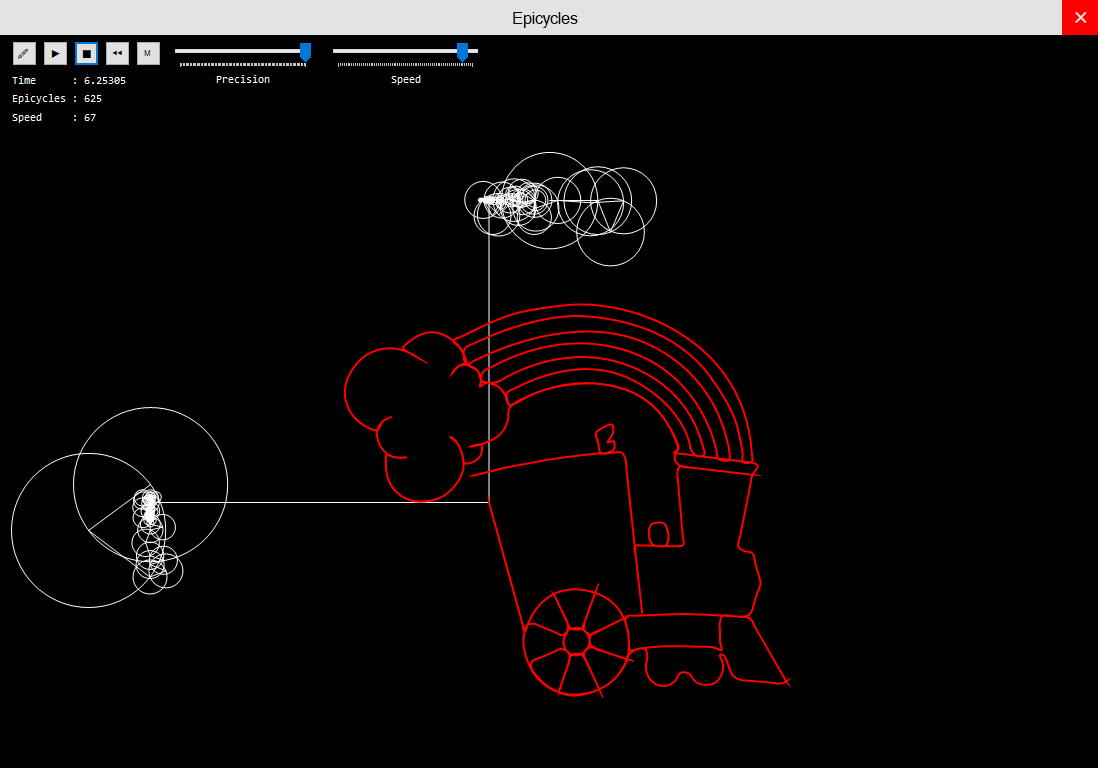
\includegraphics[scale=0.37]{images/impl1.PNG}
    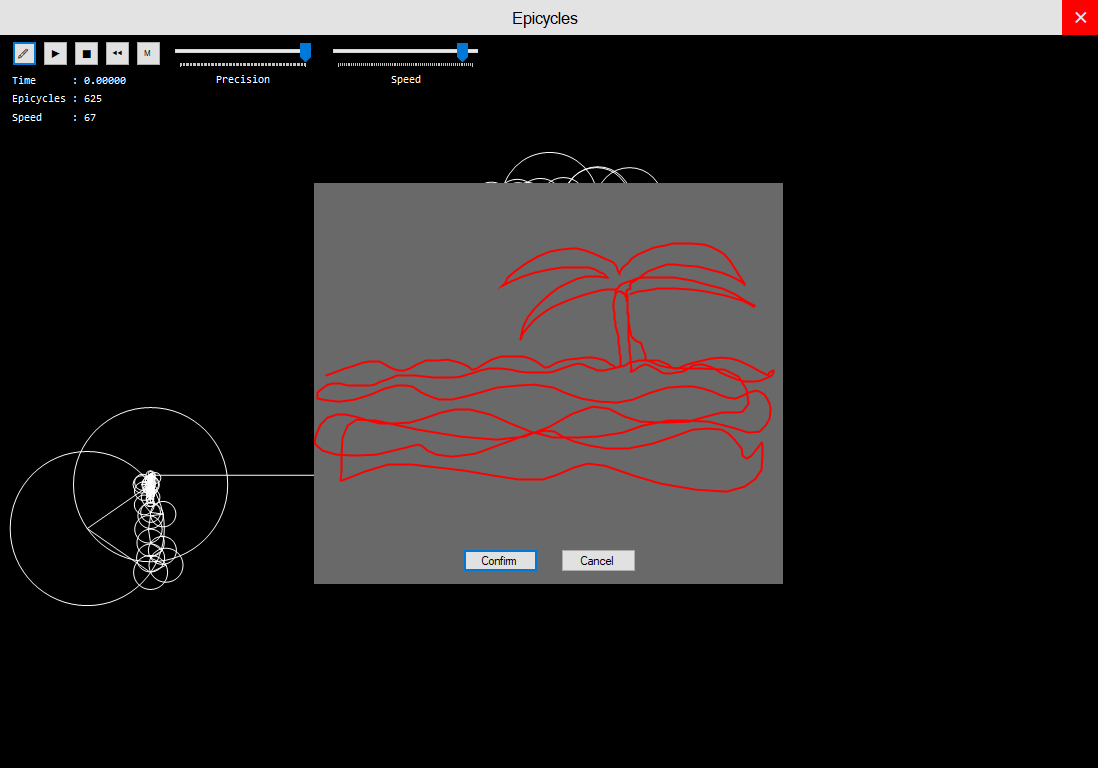
\includegraphics[scale=0.37]{images/impl2.PNG}
    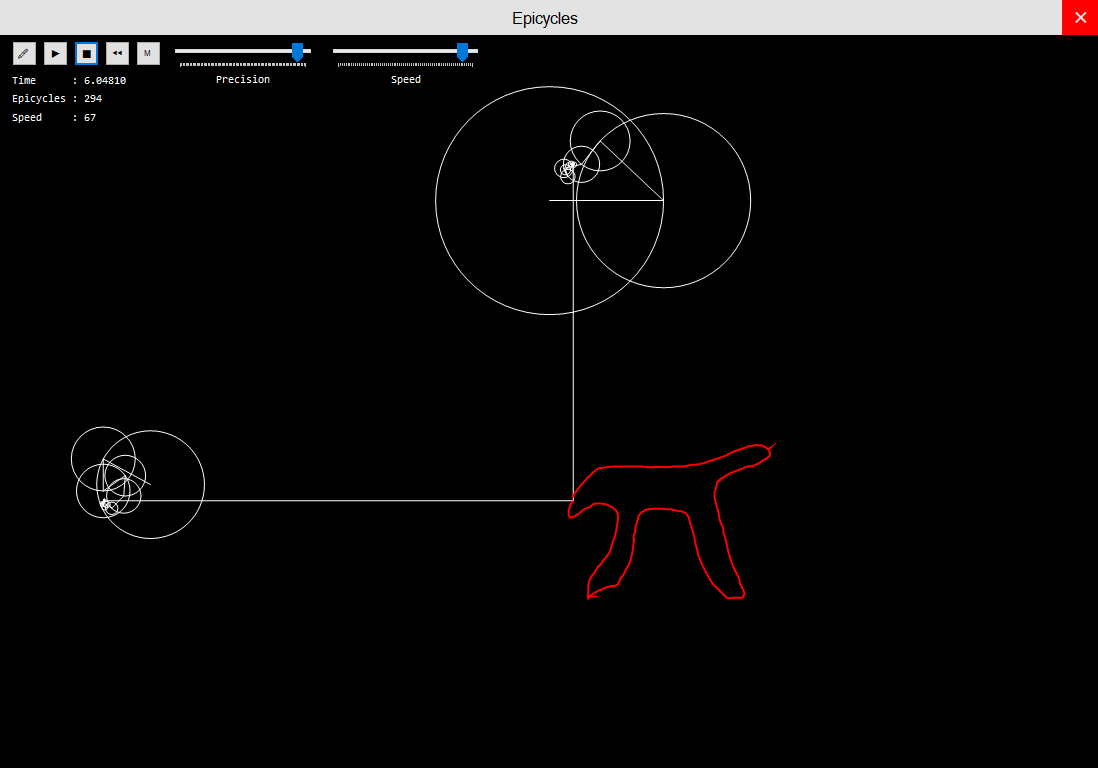
\includegraphics[scale=0.37]{images/impl3.PNG}
    \caption{Prikaz rada programa. Mogu\'c{}e je crtati proizvoljne ru\v{c}no iscrtane konture ili u\v{c}itati signal u \texttt{json} formatu.}
    \label{fig:impl}
\end{figure}



\addcontentsline{toc}{section}{Literatura}
\bibliographystyle{plain}
\bibliography{references}

\newpage

\begin{appendices}
\section{Implementacija DFT algoritma}
\label{sec:appendix:dft}

\begin{lstlisting}
public sealed class Epicycle
{
    public double Frequency { get; }
    public double Amplitude => this.value.Magnitude;
    public double Phase => this.value.Phase;
    private readonly Complex value;

    public Epicycle(int freq, Complex c)
    {
        this.value = c;
        this.Frequency = freq;
    }
}
\end{lstlisting}

\begin{lstlisting}
IReadOnlyList<Epicycle> 
DFT(IEnumerable<float> values, int? N = null) 
{
    var ys = values.ToList();
    if (N is null || N < 1)
        N = ys.Count;
    var dft = new List<Epicycle>(N.Value);

    for (int i = 0; i < N; i++) {
        double re = 0, im = 0;

        for (int n = 0; n < ys.Count; n++) {
            double phi = 2 * Math.PI * i * n / ys.Count;
            re += ys[n] * Math.Cos(phi);
            im -= ys[n] * Math.Sin(phi);
        }

        dft.Add(
            new Epicycle(
                i, 
                new Complex(
                    re / ys.Count, 
                    im / ys.Count
                )
            )
        );
    }

    return dft
        .OrderByDescending(c => c.Amplitude)
        .ToList()
        .AsReadOnly()
        ;
}
\end{lstlisting}
\end{appendices}

\end{document}
